When it comes to executing tests, there are two important things to bear in mind when working with \jb{}:
\begin{itemize}
\item All the necessary keywords for a single \bxname{use case} should be grouped together in one \gdcase{}, which is named after the use case it tests. The use case should be complete -- it should not require any data or component names. This makes it much easier to add and remove whole use cases from \gdsuites{}.   
\item Each use case should assume a well-defined state of the \gdaut{} and leave the \gdaut{} in a well-defined state. This is important for error handling later. It is a good idea to create a keyword called \bxname{app\_startup} which creates the right state for the \gdaut{}, and to use this keyword at the beginning of each use case (\bxfigref{UseCase}). 
\bxtipp{The well-defined state of your \gdaut{} may be completely empty, or may contain test data. Deciding what data your test needs and what data it will create itself is an important part of an automation strategy.}
\end{itemize}

%% \begin{figure}[h]
%% \begin{center}
%% 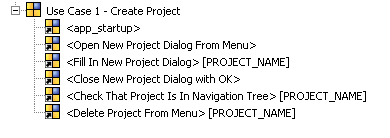
\includegraphics{BestPractices/Keywords/PS/UseCase}
%% \caption{Example Use Case}
%% \label{UseCase}
%% \end{center}
%% \end{figure} 

Use cases are then grouped together into \gdsuites{}. The \jb{} team uses the following \gdsuites{} in their tests:
\begin{itemize}
\item FULLTEST
\item FULLTEST\_BROKEN
\item WORK\_(INITIALS)
\end{itemize}

The FULLTEST \gdsuite{} contains all of the executable \bxname{Use Cases} from the \gdproject{}. There can also be \gdcases{} which reproduce errors from the bug-tracking system, called \bxname{ticket tests}. Each ticket \gdcase{} is named with the ticket number to link it to the bug-tracking system (\bxfigref{TestSuiteStructure}). 


%% \begin{figure}[h]
%% \begin{center}
%% 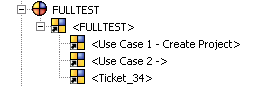
\includegraphics{BestPractices/Keywords/PS/TestSuiteStructure}
%% \caption{\gdsuite{} Structure}
%% \label{TestSuiteStructure}
%% \end{center}
%% \end{figure} 

The FULLTEST\_BROKEN \gdsuite{} contains any use cases which are currently broken and which have been removed from the FULLTEST so as not to affect any test reports or statistics. Put tests in the broken \gdsuite{} if they have been broken for some time. Tests that are critical, or which should be fixed in the next build, can be left in the FULLTEST \gdsuite{}. 

The WORK \gdsuites{} can be used by testers as a sandbox to execute single use cases during specification, or to replay tests with the intention of watching the execution. 
